\documentclass[12pt,a4paper]{article}
\usepackage[utf8]{inputenc}
\usepackage[T1]{fontenc}
\usepackage[brazil]{babel}
\usepackage{amsmath}
\usepackage{amsfonts}
\usepackage{amssymb}
\usepackage{graphicx}
\graphicspath{{images/}}
\usepackage{booktabs}
\usepackage{geometry}
\usepackage{hyperref}
\usepackage{float}
\usepackage{caption}
\usepackage{subcaption}
\usepackage{setspace}

% ─── Configurações de Layout ──────────────────────────────────────────────────
\geometry{a4paper, left=3cm, right=2cm, top=3cm, bottom=2cm}
\onehalfspacing

\begin{document}

% ─── Capa Corrigida e Formatada ───────────────────────────────────────────────
\begin{titlepage}
    \centering
    \vfill
    {\Large \textbf{Universidade Federal de Santa Maria}} \\[0.4cm]
    {\large \textbf{Centro de Tecnologia}} \\[0.4cm]
    {\large \textbf{Curso de Ciência da Computação}} \\[3cm]
    
    {\Large \textbf{Trabalho Prático: Redes Neurais Artificiais}} \\[0.5cm]
    {\large Pipeline de Machine Learning para Predição e Análise de Diabetes} \\[4cm]
    
        \textbf{Disciplina:} Inteligência Artificial \\
        \textbf{Acadêmicos:} \\
        Lucas Xavier Pairé \\
        Miguel Brondani
    
    \vfill
    {\large Santa Maria, RS} \\
    {\large \today}
    \vfill
\end{titlepage}

\newpage
\tableofcontents
\newpage

% ══════════════════════════════════════════════════════════════════════════════
\section{Introdução}
% ══════════════════════════════════════════════════════════════════════════════
Este relatório apresenta o desenvolvimento de um pipeline de Machine Learning para a predição de Diabetes Mellitus utilizando o dataset \textit{Diabetes Health Indicators} (BRFSS 2015 do CDC). O trabalho aborda classificação binária, classificação multiclasse e regressão usando redes neurais do tipo \textit{Multi-Layer Perceptron} (MLP). Foram aplicadas técnicas de amostragem estratificada, seleção de atributos por Informação Mútua (\textit{Mutual Information}), otimização de hiperparâmetros com o \textit{Optuna} e regularização por \textit{Early Stopping}. A análise foca nos impactos do desbalanceamento de classes nas métricas de avaliação e nos efeitos da redução de dimensionalidade no desempenho dos modelos.

% ══════════════════════════════════════════════════════════════════════════════
\section{Etapa 1 - Escolha e Análise do Dataset}
% ══════════════════════════════════════════════════════════════════════════════
O dataset escolhido é o \textbf{Diabetes Health Indicators Dataset}, obtido no Kaggle. Os dados vêm do \textit{Behavioral Risk Factor Surveillance System} (BRFSS) de 2015, uma pesquisa telefônica realizada anualmente pelo CDC dos Estados Unidos. O conjunto foi selecionado por conter registros sobre fatores socioeconômicos e comportamentais associados ao diabetes, sendo bastante utilizado na literatura da área.

\subsection{Características Estruturais}
O arquivo original (\textit{diabetes\_binary\_health\_indicators\_BRFSS2015.csv}) possui as seguintes especificações dimensionais primárias:
\begin{itemize}
    \item \textbf{Quantidade Total de Amostras:} 253.680 registros estruturados.
    \item \textbf{Quantidade de Atributos Preditivos (Features):} 21 variáveis explicativas.
    \item \textbf{Variável Alvo (Target):} \texttt{Diabetes\_binary}, indicando se o indivíduo é saudável (0.0) ou se possui diagnóstico prévio de diabetes ou pré-diabetes (1.0).
\end{itemize}

\subsection{Distribuição de Classes e Problemas Identificados}
A análise exploratória de dados revelou alguns pontos importantes que exigiram tratamento posterior:
\begin{itemize}
    \item \textbf{Desbalanceamento de Classes:} A variável alvo é muito desbalanceada: 86,06\% das amostras pertencem à classe 0 (saudável) e 13,94\% à classe 1 (diabetes). Essa assimetria pode fazer com que o classificador priorize a classe majoritária.
    \item \textbf{Valores Ausentes e Outliers:} Não há dados ausentes no dataset. Como a maioria das colunas representa respostas discretas ou ordinais, a presença de outliers numéricos restringe-se à variável de IMC (\texttt{BMI}).
    \item \textbf{Duplicidade de Registros:} Foram identificadas 24.206 linhas duplicadas. Apesar de respostas idênticas serem possíveis em pesquisas de larga escala, optou-se pela remoção dessas duplicatas.
    \item \textbf{Correlação Elevada:} A correlação de Pearson (Figura \ref{fig:pearson}) mostrou uma correlação linear baixa entre as variáveis de entrada e o alvo, o que justifica o uso de modelos capazes de capturar relações não-lineares, como as redes neurais.
\end{itemize}

\begin{figure}[H]
    \centering
    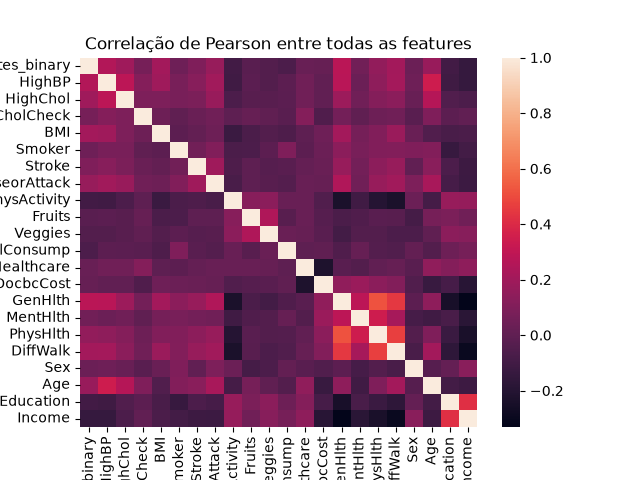
\includegraphics[width=0.65\textwidth]{full_pearson.png}
    \caption{Matriz de Correlação Linear de Pearson para os atributos do dataset.}
    \label{fig:pearson}
\end{figure}

% ══════════════════════════════════════════════════════════════════════════════
\section{Etapa 2 - Pré-processamento}
% ══════════════════════════════════════════════════════════════════════════════
Para treinar as redes MLP de forma eficiente, aplicou-se o seguinte fluxo de pré-processamento:

\subsection{Amostragem Estratificada}
Dado o tamanho do dataset (253.680 registros), o processo de treinamento repetido para busca de hiperparâmetros seria demorado. Assim, extraímos uma subamostra estratificada de 20\% do total (50.736 linhas). A estratificação manteve a proporção original de 86,06\% para a classe 0 e 13,94\% para a classe 1.

\subsection{Divisão em Treino e Teste (Holdout)}
A subamostra foi dividida em:
\begin{itemize}
    \item \textbf{80\% para Treinamento:} Usado no ajuste de pesos da rede.
    \item \textbf{20\% para Teste:} Reservado para a avaliação final do modelo com dados novos.
\end{itemize}

\subsection{Padronização de Atributos}
Como os algoritmos baseados em descida de gradiente são sensíveis à escala das variáveis, aplicou-se a padronização Z-score (\texttt{StandardScaler}) nas entradas. Isso transforma as features para terem média zero e variância unitária, evitando que atributos com valores maiores (como \texttt{BMI}) dominem o gradiente sobre atributos binários (como \texttt{Smoker}). O scaler foi ajustado no conjunto de treino e aplicado no teste para evitar vazamento de dados (\textit{data leakage}).

% ══════════════════════════════════════════════════════════════════════════════
\section{Etapa 3 - Seleção de Atributos (Feature Selection)}
% ══════════════════════════════════════════════════════════════════════════════
Para reduzir o custo computacional e mitigar overfitting, aplicamos a seleção de atributos via \textbf{Informação Mútua (Mutual Information)}. Esse método avalia a relevância das variáveis independentemente do algoritmo de aprendizado.

A Informação Mútua mede a quantidade de informação compartilhada entre duas variáveis usando a Entropia de Shannon. Diferente do coeficiente de Pearson, ela consegue capturar dependências não-lineares, o que é útil para redes neurais.

Definimos um corte para selecionar os \textbf{10 atributos com maior relevância}. Variáveis como percepção geral de saúde (\texttt{GenHlth}), Pressão Alta (\texttt{HighBP}), Colesterol Elevado (\texttt{HighChol}) e Índice de Massa Corporal (\texttt{BMI}) ficaram no topo do ranking, condizendo com os principais fatores de risco conhecidos para o diabetes.

% ══════════════════════════════════════════════════════════════════════════════
\section{Etapa 4 - Classificação com MLP}
% ══════════════════════════════════════════════════════════════════════════════

\subsection{Classificação Binária}
Como modelo \textit{baseline}, configuramos uma rede \texttt{MLPClassifier} com hiperparâmetros iniciais fixos:
\begin{itemize}
    \item \textbf{Arquitetura das Camadas Ocultas:} Duas camadas densas dispostas em formato piramidal com $(64, 32)$ neurônios, respectivamente. Esta escolha justifica-se pela busca de extrair abstrações não-lineares progressivas a partir das variáveis de entrada. O design em formato de pirâmide (reduzindo a dimensão da camada 1 para a 2) atua como um compressor de características antes da camada de saída. Além disso, o número de neurônios (totalizando aproximadamente 3.000 parâmetros ajustáveis) previne o sobreajuste em relação ao tamanho da amostra, mantendo capacidade representativa.
    \item \textbf{Função de Ativação:} Unidade Linear Retificada (\texttt{relu}), minimizando o problema de desvanecimento do gradiente e acelerando o treino.
    \item \textbf{Algoritmo Otimizador:} \texttt{adam}, devido ao cálculo computacional adaptativo de taxas de aprendizado.
    \item \textbf{Tamanho do Lote (Batch Size):} 128 instâncias por iteração.
    \item \textbf{Limitação de Épocas:} \texttt{max\_iter=150} iterações de salvaguarda.
    \item \textbf{Regularização Prematura:} Desativada temporariamente (\texttt{early\_stopping=False}).
\end{itemize}

O experimento consistiu em comparar dois cenários:
\begin{enumerate}
    \item \textbf{Cenário A (Todas as Features):} Alimentado com todos os 21 atributos originais.
    \item \textbf{Cenário B (Features Selecionadas):} Alimentado apenas com o subconjunto de 10 atributos via Informação Mútua.
\end{enumerate}

As matrizes de confusão obtidas nos testes para ambos os cenários estão na Figura \ref{fig:cm_baselines}. As métricas detalhadas são comparadas na Tabela \ref{tab:resultados_classificacao} na Etapa 6.

\begin{figure}[H]
    \centering
    \begin{subfigure}[b]{0.45\textwidth}
        \centering
        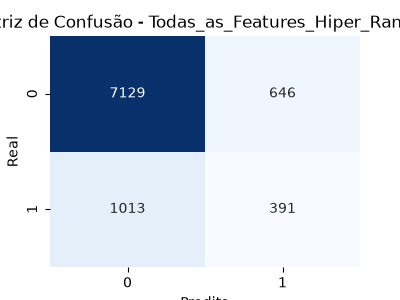
\includegraphics[width=\textwidth]{Todas_as_Features_Hiper_Random.png}
        \caption{Cenário A - Todas as Features}
        \label{fig:cm_baseline_all}
    \end{subfigure}
    \hfill
    \begin{subfigure}[b]{0.45\textwidth}
        \centering
        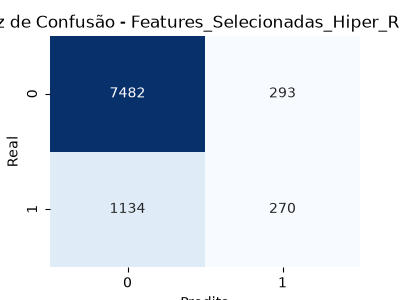
\includegraphics[width=\textwidth]{Features_Selecionadas_Hiper_Random.png}
        \caption{Cenário B - Features Selecionadas}
        \label{fig:cm_baseline_sel}
    \end{subfigure}
    \caption{Matrizes de Confusão para a MLP de Classificação Binária Baseline.}
    \label{fig:cm_baselines}
\end{figure}

% ──────────────────────────────────────────────────────────────────────────────
\subsection{Classificação Multiclasse}
% ──────────────────────────────────────────────────────────────────────────────
Para estender a análise, avaliamos a classificação de 3 classes usando o arquivo \textit{diabetes\_012\_health\_indicators\_BRFSS2015.csv}, onde a variável alvo \texttt{Diabetes\_012} indica se o indivíduo é saudável (0.0), pré-diabético (1.0) ou diabético (2.0).

O pré-processamento (holdout 80/20, amostragem de 20\% e padronização) e os 10 atributos de entrada foram mantidos. A \texttt{MLPClassifier} foi configurada com a mesma estrutura de camadas $(64, 32)$, ativação \texttt{relu} e otimizador \texttt{adam}.

A avaliação do modelo nos dados de teste gerou as seguintes métricas macro-ponderadas:
\begin{itemize}
    \item \textbf{Acurácia Global:} 0,8353
    \item \textbf{Precisão Macro:} 0,4730
    \item \textbf{Recall Macro:} 0,3814
    \item \textbf{F1-Score Macro:} 0,3882
\end{itemize}

\begin{figure}[H]
    \centering
    \begin{subfigure}[b]{0.48\textwidth}
        \centering
        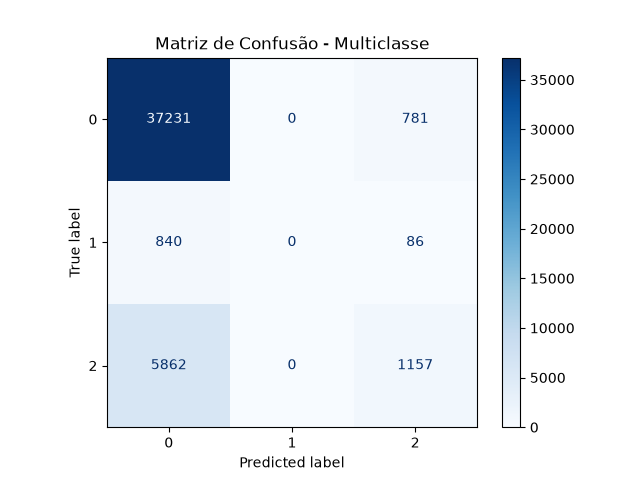
\includegraphics[width=\textwidth]{Matriz_Confusao_Multiclasse.png}
        \caption{Matriz de Confusão Multiclasse}
        \label{fig:cm_multiclass}
    \end{subfigure}
    \hfill
    \begin{subfigure}[b]{0.48\textwidth}
        \centering
        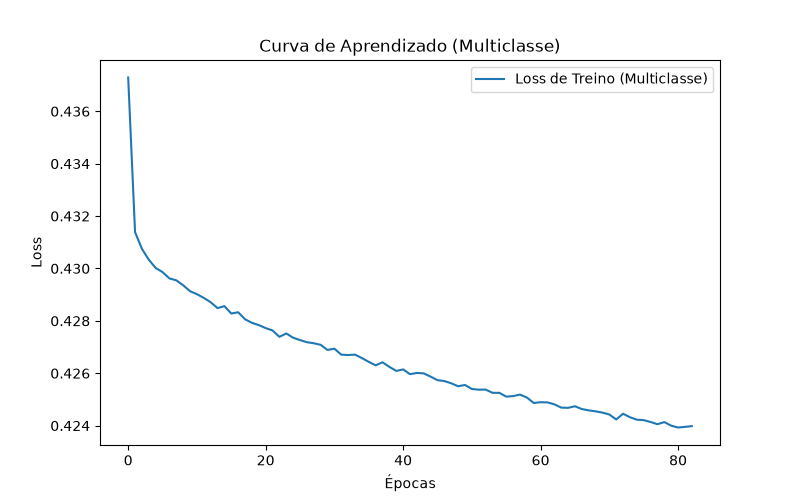
\includegraphics[width=\textwidth]{Curva_Aprendizado_Multiclasse.png}
        \caption{Curva de Aprendizado (Multiclasse)}
        \label{fig:loss_multiclass}
    \end{subfigure}
    \caption{Resultados obtidos para a MLP na tarefa de Classificação Multiclasse.}
    \label{fig:multiclass_results}
\end{figure}

A análise da matriz de confusão (Figura \ref{fig:cm_multiclass}) revela que o modelo apresenta grande facilidade para classificar corretamente indivíduos saudáveis (Classe 0), porém exibe dificuldades agudas na identificação das classes 1 (pré-diabetes) e 2 (diabetes). Essa dificuldade é explicada pelo desbalanceamento severo das classes: a classe 1 representa uma fração extremamente ínfima do conjunto de dados original (cerca de 1,8\%), fazendo com que o classificador praticamente ignore essa classe em suas predições e a confunda constantemente com as classes adjacentes. Isso prejudica o \textit{Recall} e a \textit{Precisão} macro-ponderados. A curva de perda (Figura \ref{fig:loss_multiclass}) aponta uma convergência estável da rede até o limite de 150 épocas.

% ══════════════════════════════════════════════════════════════════════════════
\section{Etapa 5 - Regressão com MLP}
% ══════════════════════════════════════════════════════════════════════════════
Adaptamos o pipeline para uma tarefa de regressão usando a classe \texttt{MLPRegressor}.

\subsection{Configuração da Meta Contínua}
A variável contínua \textbf{\texttt{BMI} (Índice de Massa Corporal)} foi removida do conjunto de entradas e redefinida como a nova variável alvo numérica contínua ($y_{reg}$). O objetivo da rede neural passou a ser a estimativa exata do IMC de um indivíduo a partir de seus demais hábitos comportamentais e indicadores clínicos (excluindo a coluna \texttt{Diabetes\_binary}). Para manter o alinhamento com a Etapa 3, o regressor foi alimentado utilizando o ranking de atributos selecionados (excetuando o próprio alvo). Os parâmetros estruturais de camadas ocultas $(64, 32)$, otimizador \texttt{adam}, ativação \texttt{relu} e \texttt{batch\_size=128} foram preservados de forma intencional para manter a consistência metodológica, permitindo uma comparação direta da capacidade de generalização e do comportamento de aprendizado da mesma arquitetura de rede neural em tarefas de natureza distinta (classificação vs. regressão).

\subsection{Resultados e Análise Crítica}
A avaliação do regressor em dados de teste inéditos gerou os seguintes resultados numéricos estáveis:
\begin{itemize}
    \item \textbf{Erro Médio Absoluto (MAE):} 4,4532
    \item \textbf{Erro Quadrático Médio (MSE):} 40,9024
    \item \textbf{Raiz do Erro Quadrático Médio (RMSE):} 6,3955
    \item \textbf{Coeficiente de Determinação ($R^2$ Score):} 0,1182
\end{itemize}

O comportamento do regressor (valores reais vs. preditos e a distribuição dos resíduos) está plotado graficamente na Figura \ref{fig:regressao_results}. A análise das métricas indica que, em média, as estimativas da MLP desviam-se por aproximadamente 4,45 pontos de IMC. O fato de o RMSE (6,3955) apresentar-se superior ao MAE (4,4532) mostra que o modelo comete erros de maior magnitude nas caudas da distribuição, demonstrando dificuldade para prever o IMC de indivíduos em extremos de peso.

O coeficiente $R^2 = 0,1182$ indica que as features de saúde disponíveis explicam apenas 11,82\% da variabilidade total do IMC. Isso reflete a complexidade do problema: fatores biológicos e comportamentais cruciais para a definição do IMC, tais como a taxa metabólica basal, o consumo calórico preciso e rotinas específicas de atividade física, não estão presentes no questionário do BRFSS, limitando o desempenho final do modelo. A evolução convergente do erro de regressão pode ser monitorada no subgráfico correspondente.

\begin{figure}[H]
    \centering
    \begin{subfigure}[b]{0.32\textwidth}
        \centering
        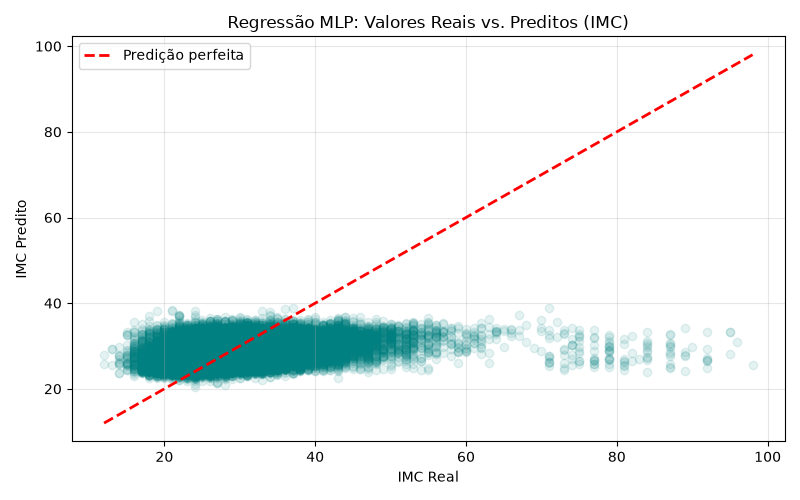
\includegraphics[width=\textwidth]{regressao_real_vs_pred.png}
        \caption{Valores Reais vs. Preditos}
        \label{fig:regressao_real_pred}
    \end{subfigure}
    \hfill
    \begin{subfigure}[b]{0.32\textwidth}
        \centering
        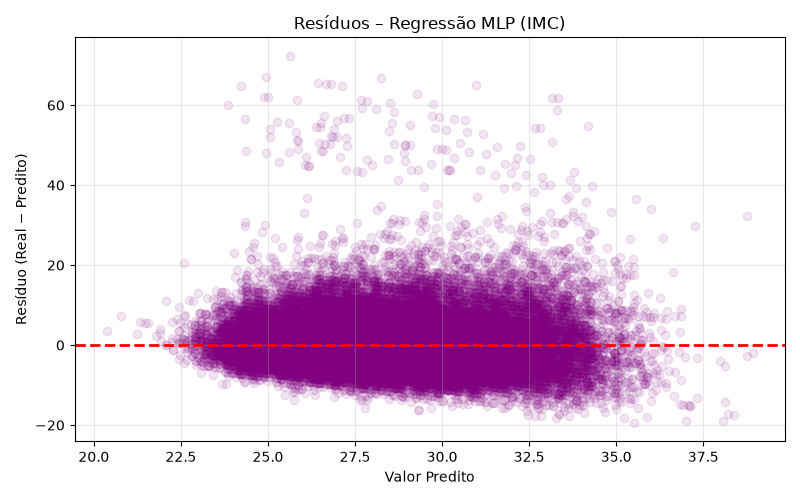
\includegraphics[width=\textwidth]{regressao_residuos.png}
        \caption{Distribuição dos Resíduos}
        \label{fig:regressao_residuos}
    \end{subfigure}
    \hfill
    \begin{subfigure}[b]{0.32\textwidth}
        \centering
        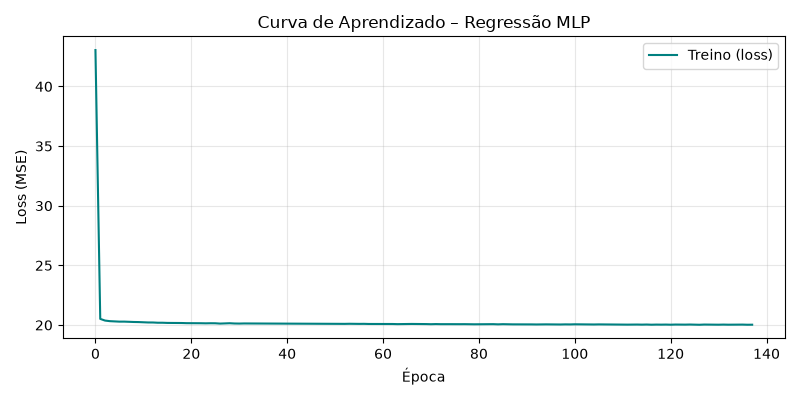
\includegraphics[width=\textwidth]{curva_aprendizado_regressao.png}
        \caption{Curva de Aprendizado (Loss)}
        \label{fig:curva_regressao}
    \end{subfigure}
    \caption{Resultados gráficos obtidos na Etapa 5 (Regressão).}
    \label{fig:regressao_results}
\end{figure}

% ══════════════════════════════════════════════════════════════════════════════
\section{Etapa 6 - Otimização de Hiperparâmetros}
% ══════════════════════════════════════════════════════════════════════════════
Retornando ao escopo da Classificação Binária, utilizamos o framework \textbf{Optuna} para buscar melhores hiperparâmetros. O foco na classificação binária se deu pelas baixas taxas de Recall observadas nas redes baseline da Etapa 4, causadas pelo desbalanceamento.

\subsection{Estratégia do Espaço de Busca e Função Objetivo}
O Optuna utilizou amostragem bayesiana (algoritmo TPE) em 10 trials no seguinte espaço dinâmico:
\begin{itemize}
    \item Neurônios na Camada Oculta 1: Inteiros entre 32 e 128 (passo de 32).
    \item Neurônios na Camada Oculta 2: Inteiros entre 16 e 64 (passo de 16).
    \item Função de Ativação: Alternância entre \texttt{relu} e \texttt{tanh}.
    \item Taxa de Aprendizado Inicial ($\alpha$): Escala logarítmica contínua entre $10^{-4}$ e $10^{-2}$.
    \item Tamanho do Lote (\textit{Batch Size}): Escolha categórica entre $[64, 128, 256]$.
\end{itemize}

A função objetivo buscou maximizar o F1-Score no conjunto de validação para forçar a rede a reduzir falsos negativos. O classificador final otimizado foi reavaliado e sua matriz de confusão correspondente gerada (Figura \ref{fig:cm_optuna}).

\begin{figure}[H]
    \centering
    \includegraphics[width=0.4\textwidth]{{MLP Otimizada (Optuna)}.png}
    \caption{Matriz de Confusão do modelo MLP Otimizado via Optuna.}
    \label{fig:cm_optuna}
\end{figure}

\subsection{Tabela Comparativa Geral do Pipeline}
A Tabela \ref{tab:resultados_classificacao} consolida o desempenho evolutivo observado ao longo do projeto para a classificação binária, incluindo os dados obtidos após a aplicação de regularização discutidos na seção seguinte.

\begin{table}[H]
\centering
\caption{Métricas Comparativas de Desempenho (Classificação Binária).}
\label{tab:resultados_classificacao}
\resizebox{\textwidth}{!}{%
\begin{tabular}{cccccc}
\toprule
\textbf{Cenário / Modelo} & \textbf{Accuracy} & \textbf{Precision} & \textbf{Recall} & \textbf{F1-Score} & \textbf{ROC-AUC} \\ \midrule
Todas\_as\_Features\_Hiper\_Random & 0,819261 & 0,377049 & 0,278490 & 0,320361 & 0,750299 \\ 
Features\_Selecionadas\_Hiper\_Random & 0,844536 & 0,479574 & 0,192308 & 0,274530 & 0,775117 \\ 
MLP Otimizada (Optuna) & 0,847587 & 0,505112 & 0,175926 & 0,260961 & 0,794098 \\ 
MLP Regularizada (Early Stopping) & 0,850746 & 0,552469 & 0,127493 & 0,207176 & 0,802013 \\ \bottomrule
\end{tabular}%
}
\end{table}

\subsection{Análise Crítica dos Baixos Valores de F1-Score e Recall}
A Tabela \ref{tab:resultados_classificacao} mostra que, enquanto a acurácia é alta (entre 81,9\% e 85,1\%), as métricas que avaliam a classe positiva (Recall e F1-Score) são baixas.

Isso ocorre porque apenas 13,94\% dos dados são positivos. O classificador tende a focar na classe majoritária para reduzir o erro global. Como consequência:
\begin{enumerate}
    \item \textbf{A Ilusão da Acurácia:} Um modelo simples que apenas classificasse todos como saudáveis (classe 0) obteria cerca de 86\% de acurácia. Por isso, os altos valores de acurácia observados não refletem eficácia clínica, mas sim o peso estatístico da classe majoritária.
    \item \textbf{Subestimação do Recall (Sensibilidade):} O Recall variou entre 12,7\% e 17,6\% nos modelos otimizados e regularizados. Isso significa que a rede identifica apenas cerca de 1 em cada 6 ou 8 diabéticos, gerando muitos falsos negativos.
    \item \textbf{A Queda Consequente do F1-Score:} Como o F1-Score é a média harmônica entre Precision e Recall, ele é puxado para baixo pelo baixo Recall, limitando-se ao teto de 0,2610 (atingido pelo Optuna).
    \item \textbf{A Importância do ROC-AUC:} O ROC-AUC manteve-se estável, alcançando 0,8020 no modelo com Early Stopping. O ROC-AUC avalia a ordenação probabilística do classificador. O valor próximo a 0,80 indica que a rede aprendeu a ordenar bem as probabilidades, mas o limiar de decisão de 0,5 prejudica a classificação.
\end{enumerate}

Para aplicações clínicas, contornar esses limites exigiria ajustar o threshold de decisão via curvas ROC, usar pesos nas classes (\textit{class weights}) na função de perda, ou aplicar algoritmos de sobreamostragem (como o \textit{SMOTE}).

% ══════════════════════════════════════════════════════════════════════════════
\section{Etapa 7 - Regularização}
% ══════════════════════════════════════════════════════════════════════════════
A etapa final consistiu na aplicação de técnicas de regularização, comparando o comportamento da rede com os cenários anteriores.

\subsection{Técnica Utilizada e Configuração}
A abordagem de regularização incorporada ao projeto foi o \textbf{Early Stopping (Parada Antecipada)}. O algoritmo separa 15\% dos dados de treino para validação. Se a perda ou a acurácia de validação não melhorar por 10 épocas seguidas, o treino é interrompido para evitar overfitting.

\begin{figure}[H]
    \centering
    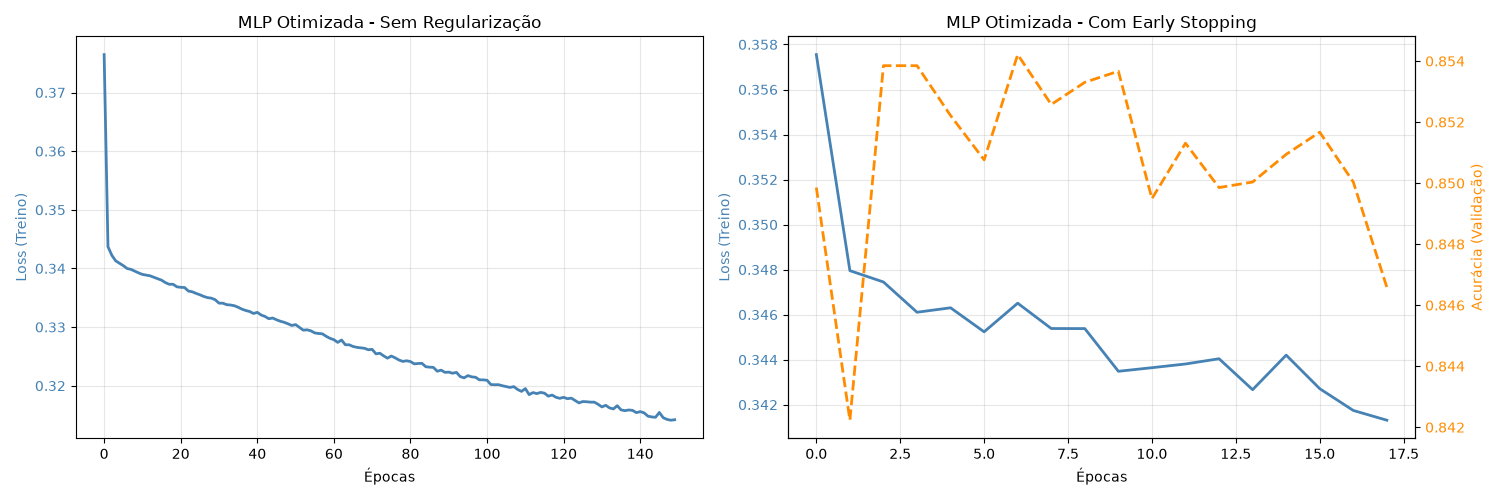
\includegraphics[width=0.75\textwidth]{overfitting_analise.png}
    \caption{Curvas de Aprendizado para os cenários Otimizado sem Regularização e com Early Stopping.}
    \label{fig:curva_aprendizado_regularizada}
\end{figure}

A Figura \ref{fig:curva_aprendizado_regularizada} ilustra os gráficos de monitoramento. Sem regularização, a perda de treino cai constantemente até o limite de épocas. Com Early Stopping, o treino é interrompido antes das 150 épocas quando a curva de validação (tracejado laranja) atinge estabilidade.

\subsection{Discussão dos Resultados}
A análise das curvas mostra que o treinamento convergiu de forma estável e que a Informação Mútua reduziu a complexidade, favorecendo a generalização.

No conjunto de teste, o modelo com Early Stopping teve um aumento de precisão, que subiu de 50,5\% para \textbf{55,2\%}, e de ROC-AUC, que chegou a \textbf{0,8020}. O Recall caiu para 12,7\% (com F1 de 0,2072), mas o modelo final se mostrou mais robusto contra falsos positivos, indicando que a parada antecipada barrou ajustes espúrios.

Considerando os resultados, o melhor equilíbrio entre desempenho e generalização foi alcançado pela combinação de seleção de atributos por Informação Mútua, otimização de hiperparâmetros com Optuna e regularização por Early Stopping.

% ══════════════════════════════════════════════════════════════════════════════
\section{Conclusão}
% ══════════════════════════════════════════════════════════════════════════════
O pipeline desenvolvido cumpriu os requisitos propostos. O estudo confirmou que a acurácia isolada é insuficiente para problemas biomédicos desbalanceados e provou que o gerenciamento correto da dimensionalidade e o ajuste fino de parâmetros via Early Stopping e Optuna ajudam a obter redes neurais mais robustas e generalistas.

\end{document}
